\begin{problem}%
{Отопление}%
{\textsl{стандартный ввод}}%
{\textsl{стандартный вывод}}%
{2 секунды}%
{256 мегабайт}{}

Дядя Федор и почтальон Печкин готовятся к холодной зиме в деревне Простоквашино. Для этого необходимо подвести отопление от котельной к домам дяди Федора и почтальона Печкина. Для удобства представим территорию Простоквашино как клетчатую сетку, причем котельная будет находиться в клетке ($0$, $0$). Дом дяди Федора расположен в клетке ($a$, $b$), а почтальона Печкина — в ($c$, $d$).

\begin{center}
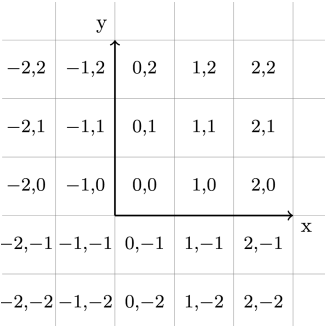
\includegraphics[scale=0.5]{images/1.png}\\
\textit{территория Простоквашино как клетчатая сетка}
\end{center}

В начале строительства считается, что отопление доведено только до клетки с котельной. Затем, каждый день рабочие могут провести теплотрассу до любой клетки, которая на текущий момент является соседней с хотя бы одной клеткой, куда отопление уже доведено. Клетки называются соседними, если касаются хотя бы в одной точке.

\begin{center}
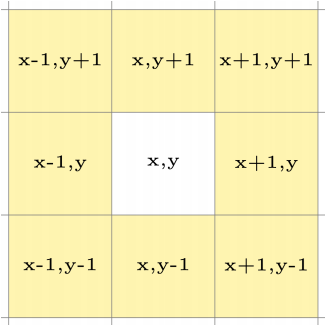
\includegraphics[scale=0.5]{images/2.png}\\
\textit{соседи клетки ($x$, $y$)}
\end{center}

Требуется написать программу, вычисляющую минимальное число дней, которое понадобится рабочим, чтобы отопить оба дома.

\InputFile

В первой строке заданы два целых числа $a$ и $b$ через пробел. Во второй строке заданы два целых числа $c$ и $d$ через пробел. Гарантируется, что все числа находятся в промежутке от $-10^4$ до $10^4$. Котельная, дом дяди Федора и дом почтальона Печкина находятся в трех разных клетках.

\OutputFile

Выведите единственное число — минимальное количество дней, которое понадобится, чтобы подвести отопление к домам дяди Федора и почтальона Печкина.

\Examples

\begin{example}
\exmp{
2 0
0 2
}{%
3
}%
\exmp{
-2 -1
-3 -2
}{%
3
}%
\end{example}

\Explanations

\begin{center}
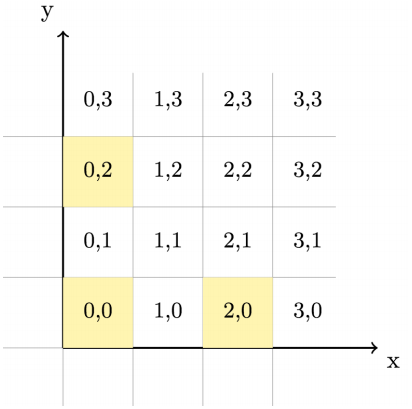
\includegraphics[scale=0.5]{images/3.png}\\
\textit{В первом тесте оптимально будет в первый день довести отопление от котельной в клетке (0, 0) до клетки (1, 1), затем в следующие два дня отопить оба дома, для
которых (1, 1) является соседней.}
\end{center}

\begin{center}
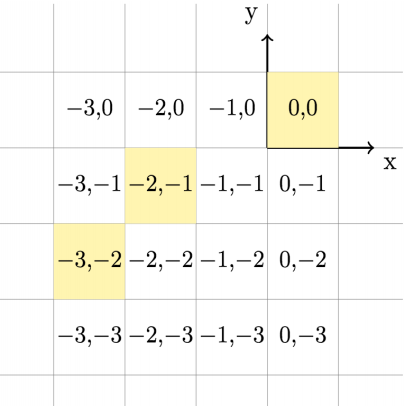
\includegraphics[scale=0.5]{images/4.png}\\
\textit{Во втором тесте возможный порядок подключения клеток к отоплению такой: (-1, -1), (-2, -1), (-3, -2).}
\end{center}

\end{problem}
